\chapter{สภาพการปฏิบัติงาน}

\section{บรรยากาศในสถานที่ปฏิบัติงาน}

ออฟฟิศของ \Company อยู่ที่ ชั้น 16 ห้อง 16บี ตึกปิยเพลส ซอยหลังสวน ถนนเพลินจิต แขวงลุมพินี มีพนักงานทั้งหมด 16 คน ซึ่งทีม Delivery ที่ผู้เขียนเข้าไปฝึกงานนั้นมีพนักงานอยู่ 14 คน พนกังานแต่ละฝ่ายจะนั่งรวมกันโดยไม่มีการฉากกั้น หรือแบ่งห้องตามแต่ละฝ่ายงาน ซึ่งเป็นลกัษณะของออฟฟิศสมัยใหม่นอกจากนี้ยังมีห้องประชุม ห้องครัว ห้องน้ำ ห้องนั่งเล่น และระเบียงที่เอาไว้ปลูกผัก

\begin{figure}[!h]
    \centering
    \subfigure[ห้องขนม]{
        \label{Fig:office:1}
        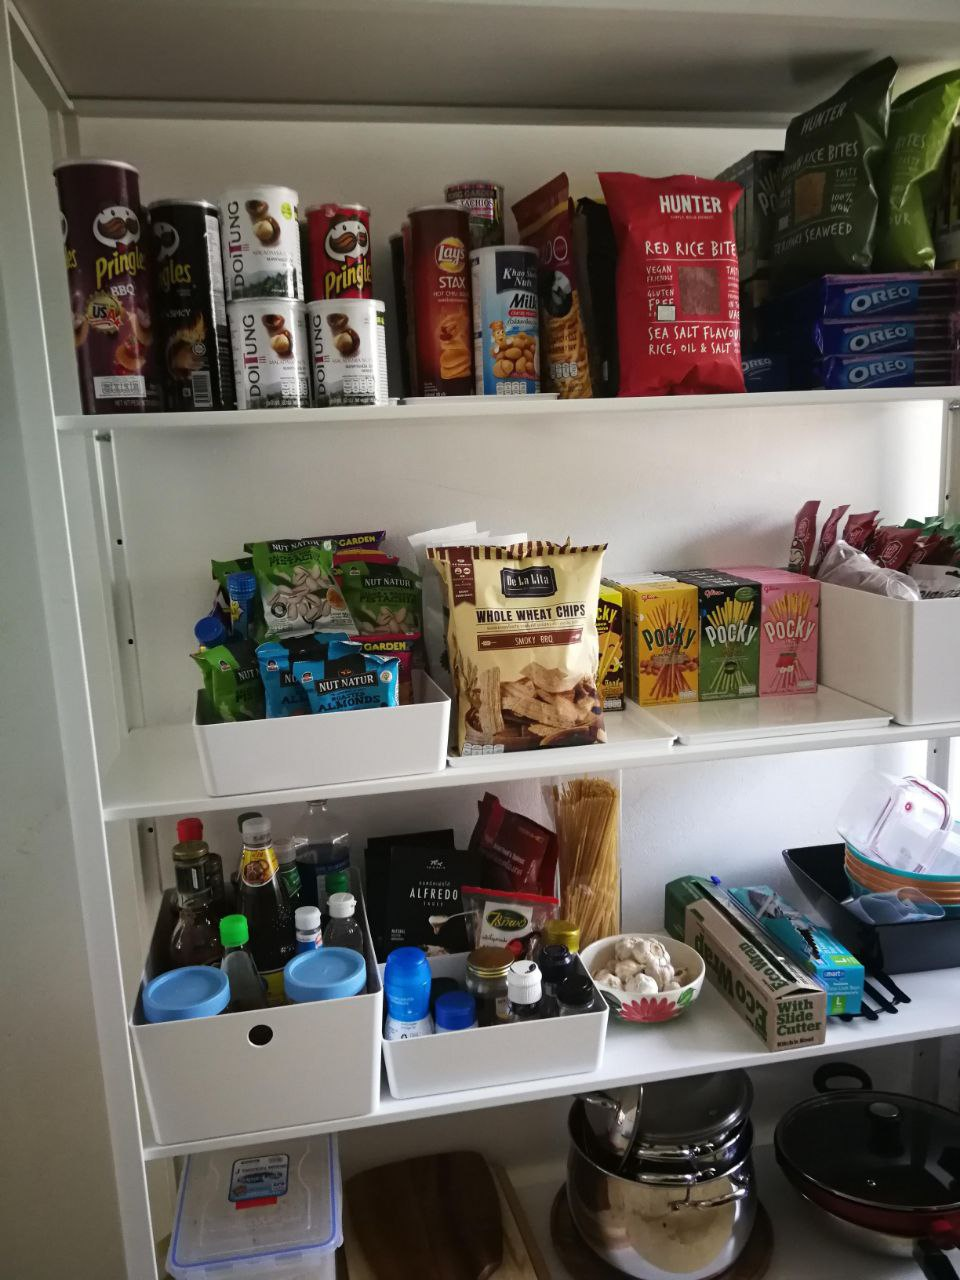
\includegraphics[width=0.45\linewidth]{snacksroom.jpeg}
    }
    \subfigure[ระเบียงปลูกผัก]{
        \label{Fig:office:2}
        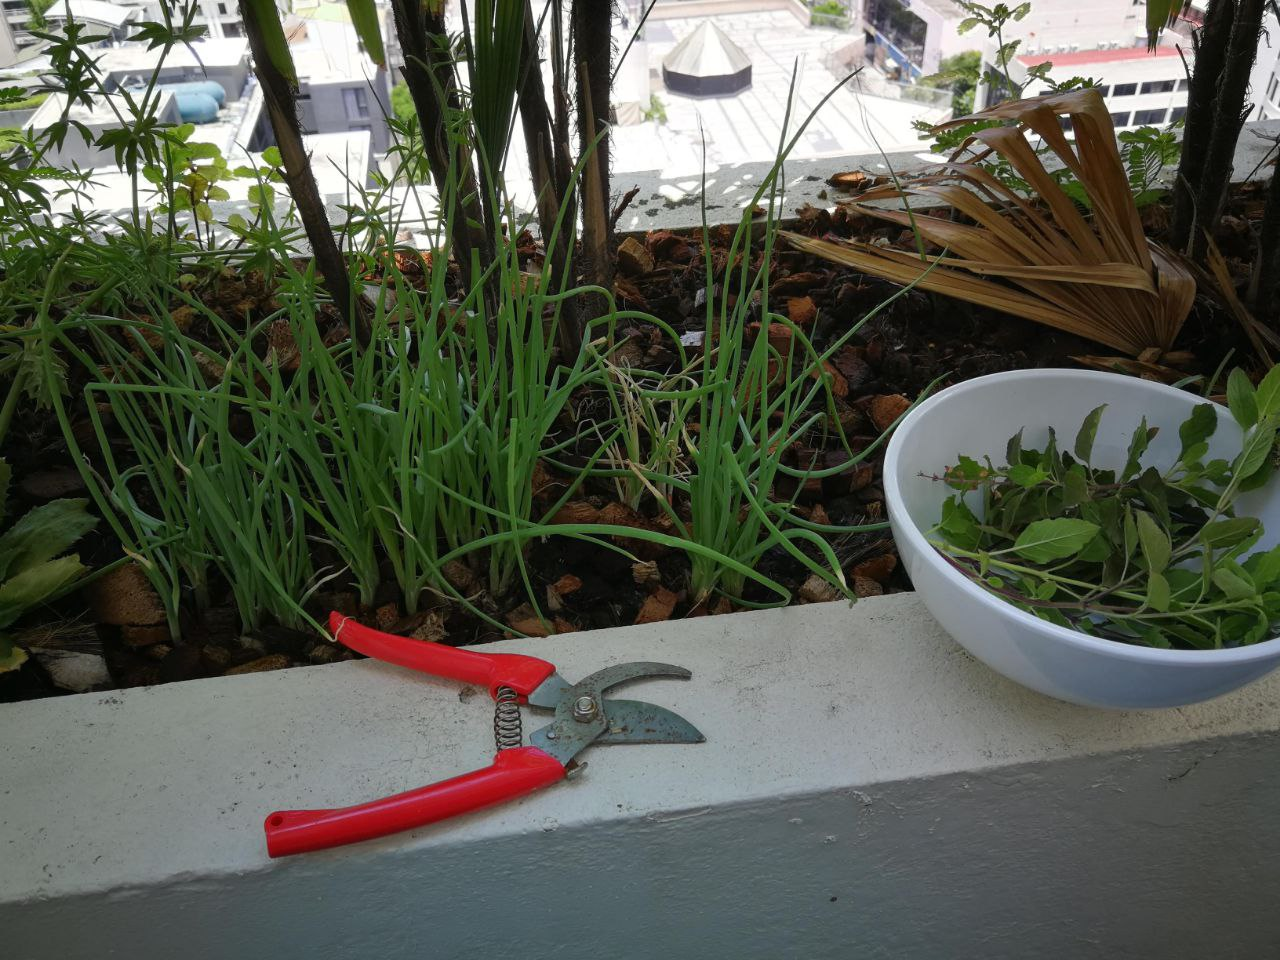
\includegraphics[width=0.45\linewidth]{balcony.jpeg}
    }
    \subfigure[ห้องครัว]{
        \label{Fig:dorm:4}
        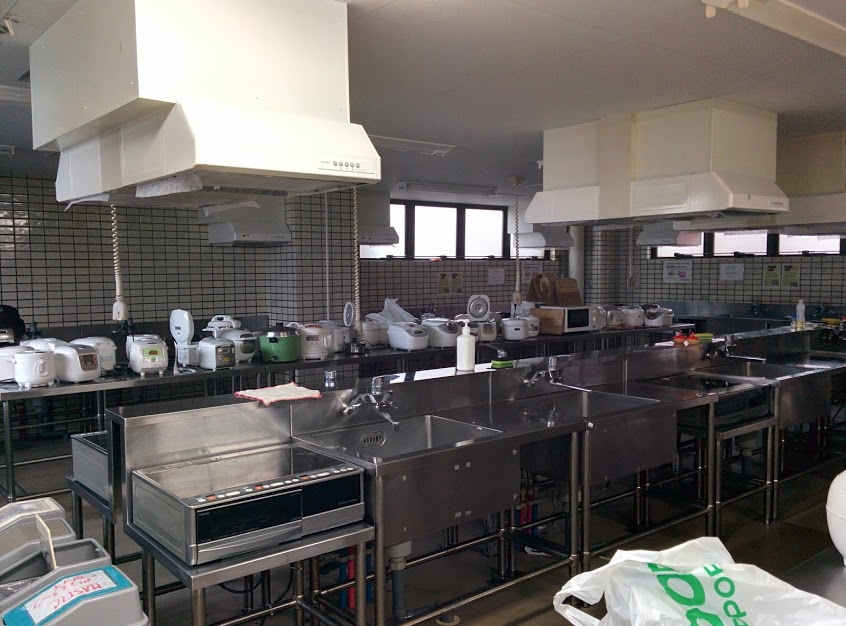
\includegraphics[width=0.45\linewidth]{dorm3}
    }
    \caption{ภาพออฟฟิศที่ทำงาน}
    \label{Fig:office}
\end{figure}

\section{กิจกรรมระหว่างฝึกงาน}

เนื่องจากในเดือนตุลาคมทางบริษัทได้จับกิจหรรมที่ชื่อว่า Team Event ซึ่งเป็นกิจกรรมที่ทุกคนในทีม Asia Pacific ประกอบ ไปทำกิจกรรมร่วมกันที่ต่างประเทศ โดยบริษัทจะออกค่าใช้จ่ายให้ทั้งหมด โดยกิจกรรมจัดขึ้นที่เกาะ Bintan ประเทศ Indonesia วันที่ 11 ตุลาคม ถึง 13 ตุลาคม พ.ศ. 2562

\begin{figure}[!h]
	\centering
	\subfigure[ห้องพัก]{
		\label{Fig:teamevent:1}
		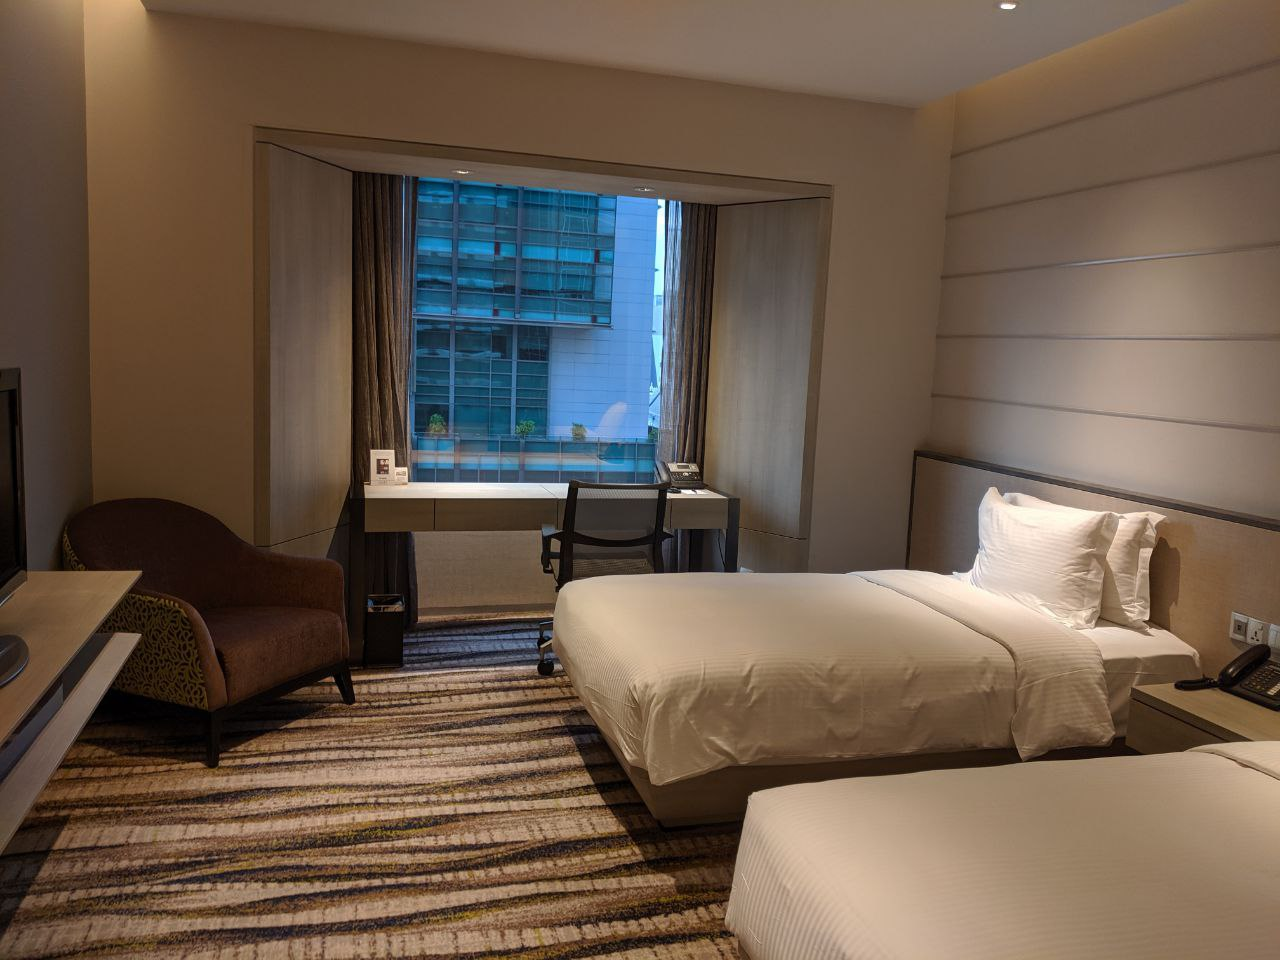
\includegraphics[width=0.45\linewidth]{room.jpeg}
	}
	\subfigure[ชายหาด ณ ที่พัก]{
		\label{Fig:teamevent:2}
		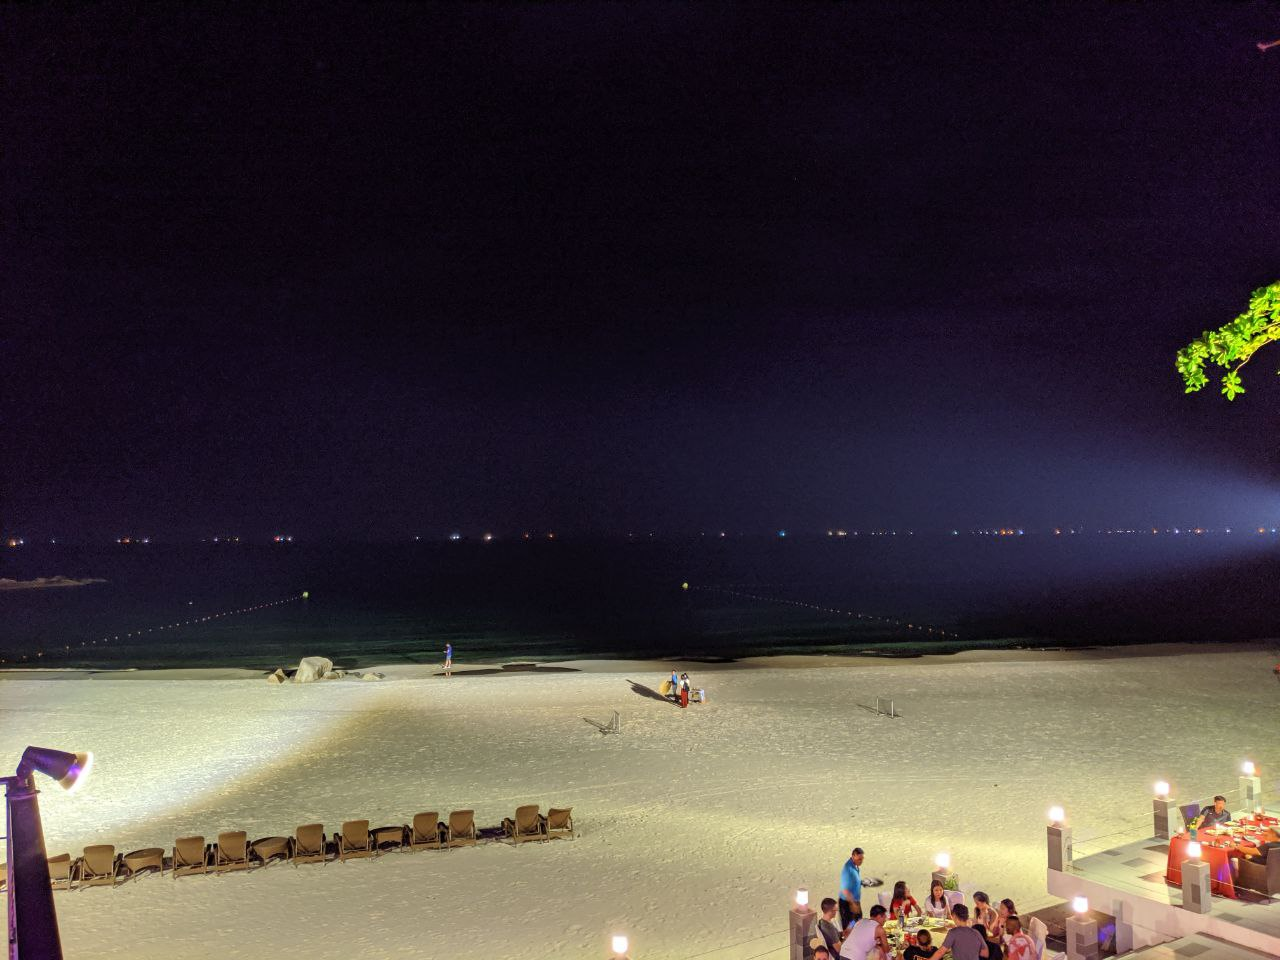
\includegraphics[width=0.45\linewidth]{bintanbeach.jpeg}
	}
	\subfigure[แข่งขันแทงพูล]{
		\label{Fig:teamevent:_}
		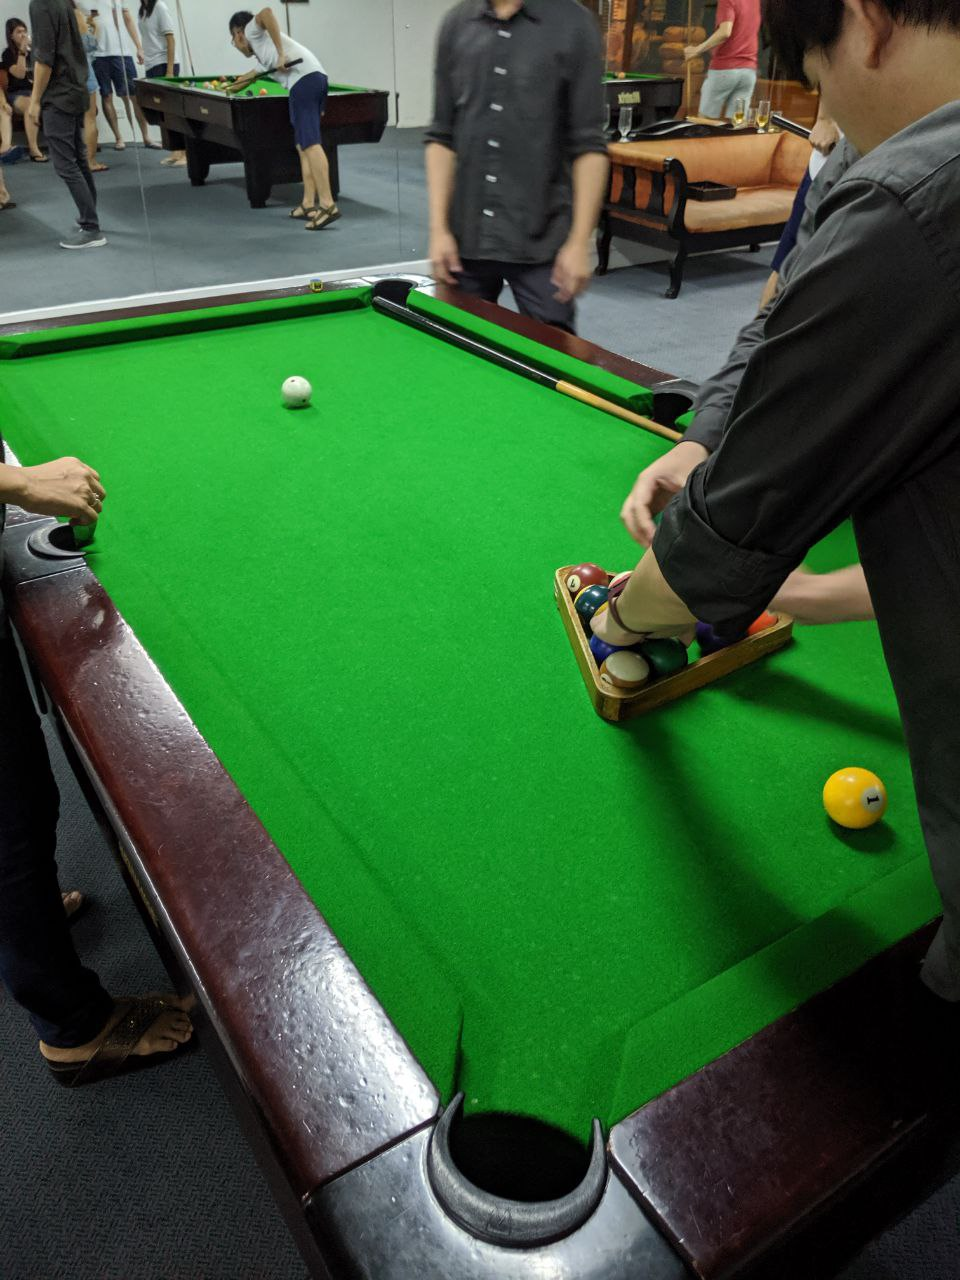
\includegraphics[height=0.35\linewidth]{bintanpool.jpeg}
	}
	\subfigure[แข่งขันกีฬาทางน้ำ]{
		\label{Fig:teamevent:4}
		\includegraphics[width=0.45\linewidth]{watersport.jpg}
	}
	\caption{ภาพกิจกรรม Team Event}
	\label{Fig:teamevent}
\end{figure}

\chapter{ประวัติผู้เขียน}

 \begin{figure}[h]
	\centering
	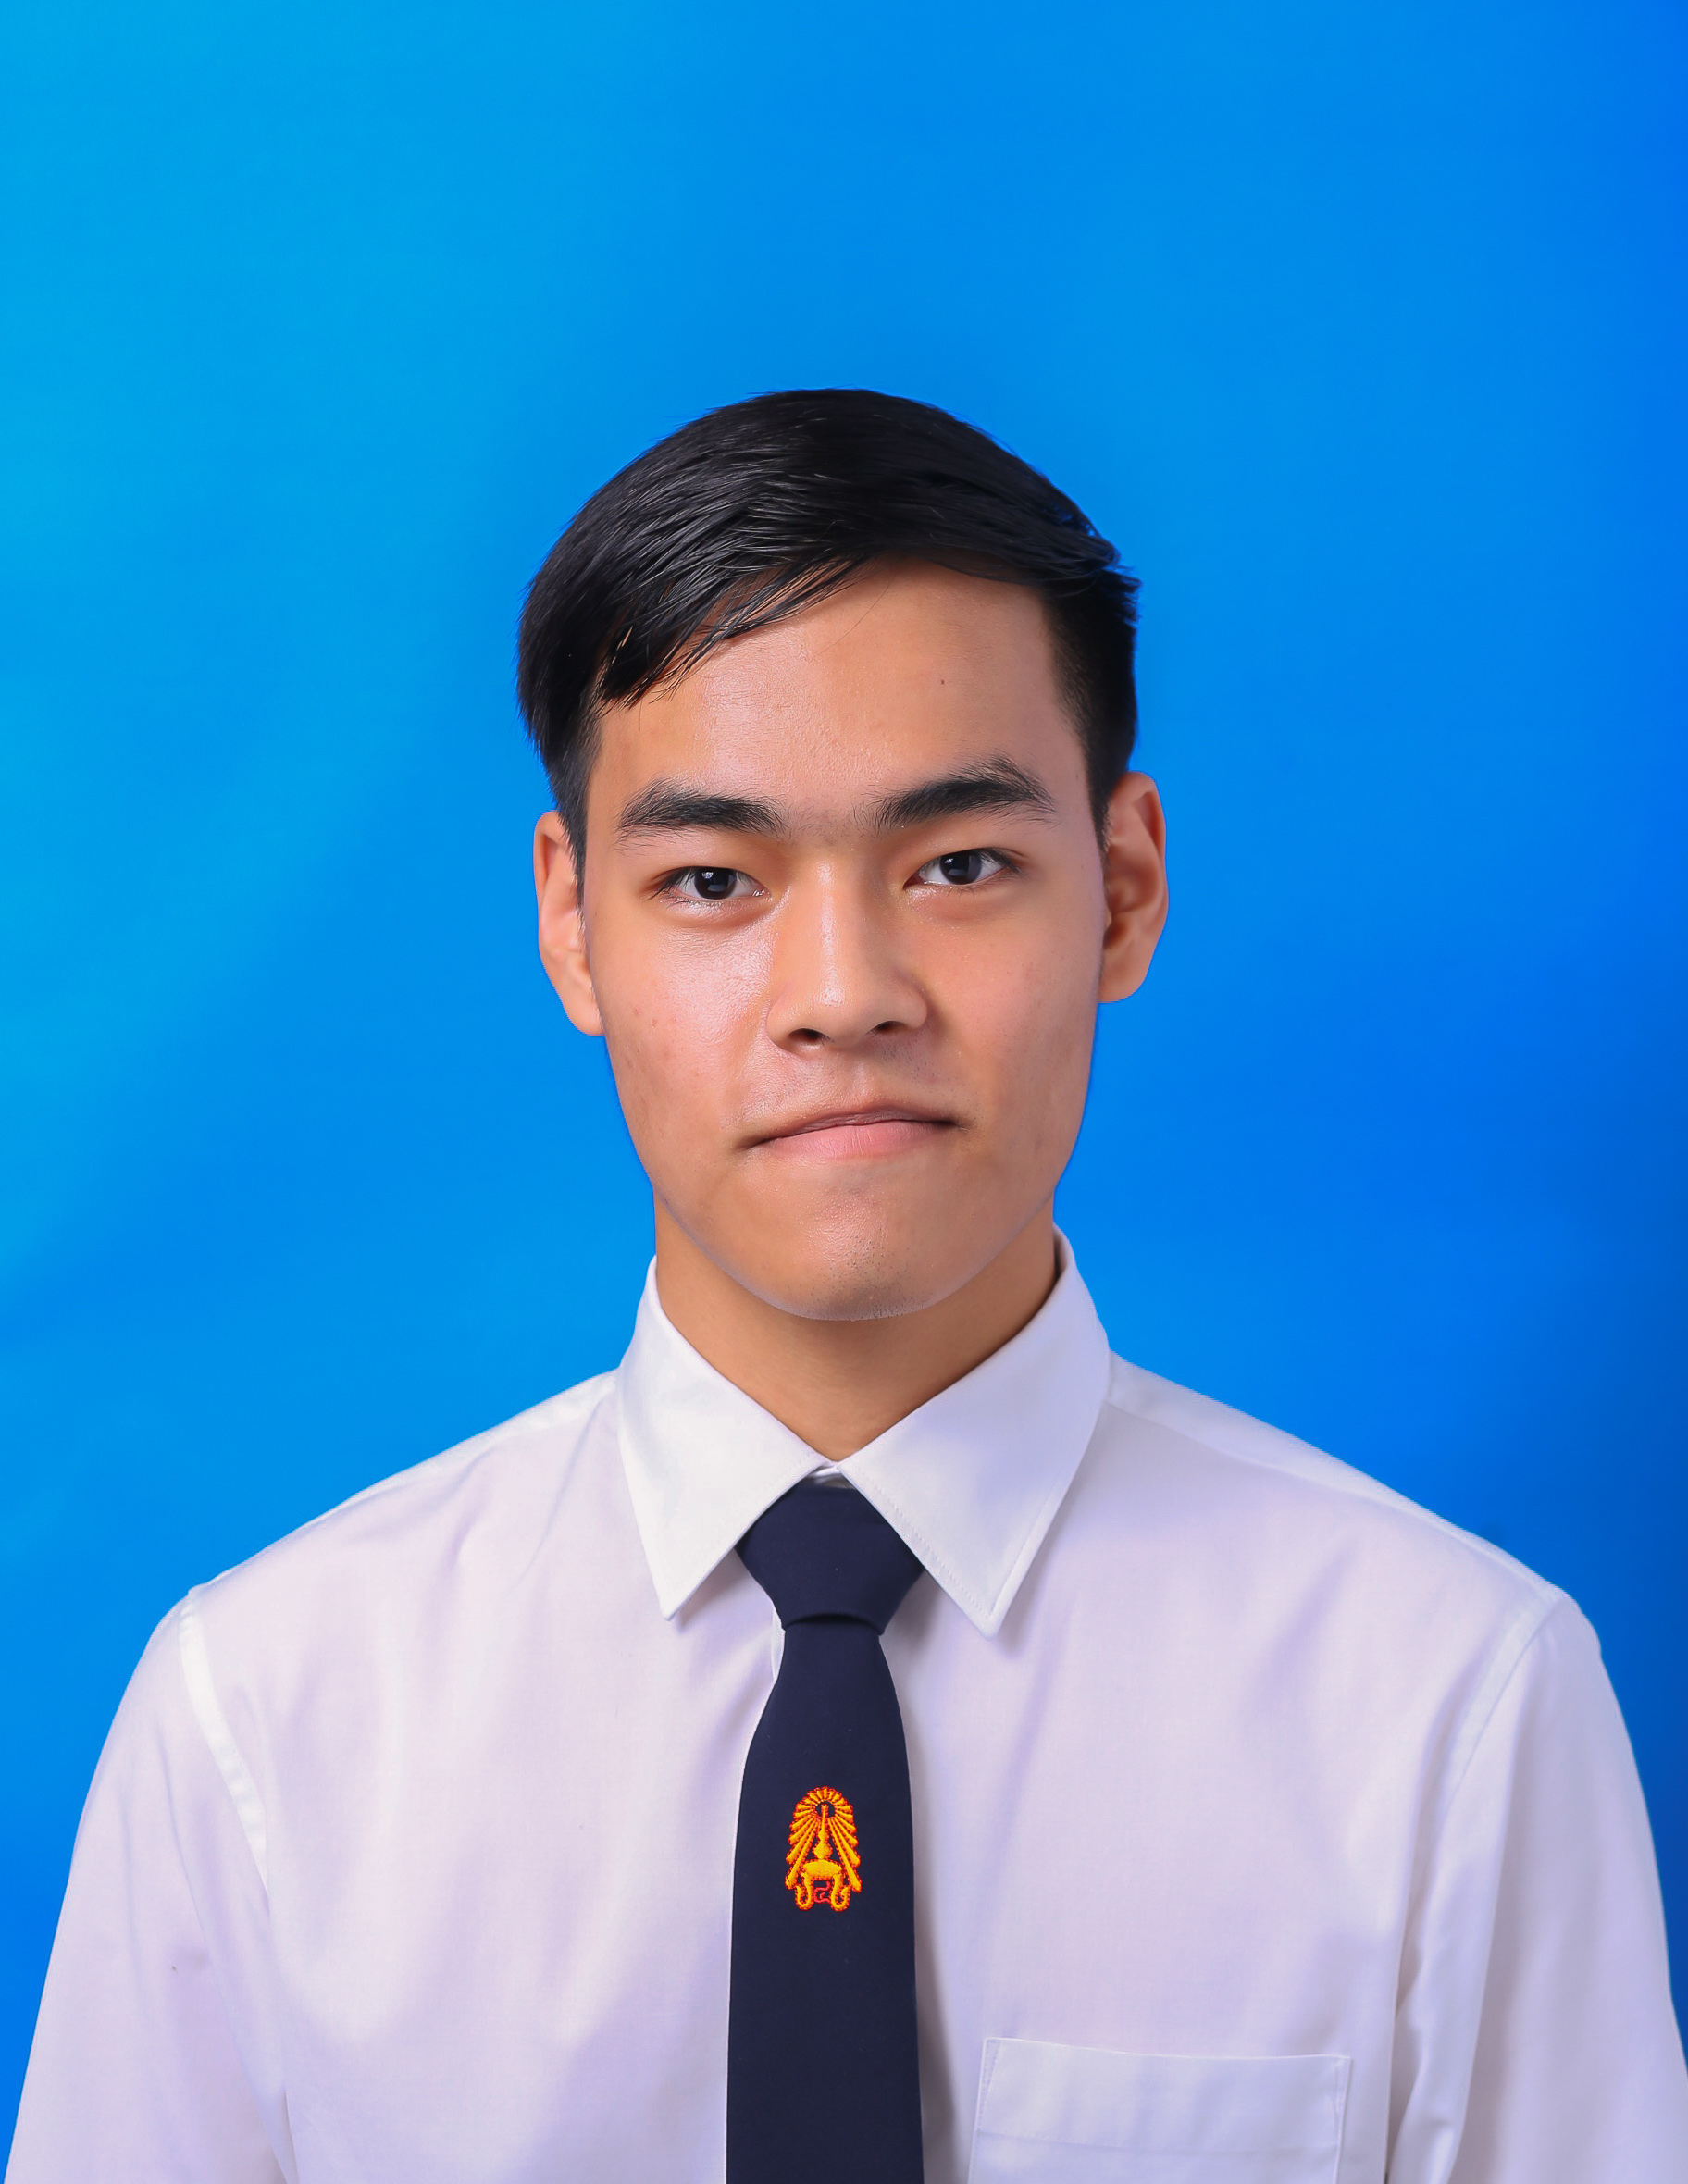
\includegraphics[width=0.3\columnwidth]{std.jpg}
	\label{Fig:std.jpg}
\end{figure}

\begin{center}

\begin{tabular}{l l}
	ชื่อ - นามสกุล & \AuName \\
	Email & weeruhputt.s@gmail.com \\
	ประวัติและผลงานเพิ่มเติม & linkedin.com/in/weeruhputt \\
\end{tabular}

\end{center}
